\subsubsection{Calibración Espacial Píxel-Milímetro}

Las desviaciones detectadas mediante el sistema de visión se expresan inicialmente en unidades de píxeles, magnitud que carece de significado físico directo para el sistema de control de movimiento. Se requiere establecer una correspondencia entre coordenadas en el plano de la imagen y coordenadas en el espacio físico del robot. Esta transformación se logra mediante un proceso de calibración que determina los factores de conversión píxel-milímetro.

La calibración se fundamenta en la geometría proyectiva de formación de imágenes. Bajo la aproximación de modelo de cámara estenopeica, existe una relación lineal entre distancias en el plano objeto (espacio físico) y distancias en el plano imagen (espacio de píxeles), siempre que la distancia focal y la distancia objeto-cámara permanezcan constantes. Esta relación se expresa mediante:

\begin{equation}
d_{mm} = K \cdot d_{px}
\end{equation}

donde $d_{mm}$ es la distancia física en milímetros, $d_{px}$ es la distancia correspondiente en píxeles, y $K$ es el factor de conversión con unidades mm/píxel.

\textbf{Metodología de Calibración}

El proceso de calibración empleó un patrón de referencia con dimensiones conocidas colocado en el plano de trabajo a la distancia nominal de 200 milímetros desde el sensor de la cámara. El patrón consistió en un conjunto de marcas separadas por distancias calibradas mediante instrumentos de metrología de precisión.

Se capturaron imágenes del patrón y se identificaron las posiciones en píxeles de las marcas de referencia mediante detección de contornos. Para cada par de marcas consecutivas se registró la distancia física conocida $d_{mm,i}$ y la distancia medida en píxeles $d_{px,i}$. Se recolectaron $N = 20$ mediciones de distancias que cubrían el rango completo del espacio de trabajo.

El factor de conversión óptimo se determinó mediante el método de mínimos cuadrados. Para el modelo lineal bivariable:

\begin{equation}
d_{mm} = k \cdot d_{px} + b
\end{equation}

donde $b$ representa un offset constante. Los parámetros se determinan resolviendo el sistema de ecuaciones normales. El análisis de los datos de calibración reveló que el offset $b$ resultó despreciable (inferior a 0.1 mm), validando la hipótesis de relación puramente proporcional entre coordenadas de píxeles y coordenadas físicas. En consecuencia, se adoptó el modelo simplificado sin offset.

\textbf{Resultados de Calibración}

Los factores de conversión obtenidos fueron:

\begin{equation}
K_x = 0.146 \text{ mm/px}
\end{equation}

\begin{equation}
K_y = 0.148 \text{ mm/px}
\end{equation}

La diferencia entre los factores en direcciones horizontal y vertical se atribuye a pequeñas distorsiones ópticas del sistema de lentes y a la geometría no perfectamente cuadrada de los píxeles del sensor CMOS. Esta diferencia del 1.4 por ciento es despreciable para la mayoría de aplicaciones, pero se mantienen factores independientes para maximizar la precisión.

La bondad de ajuste del modelo lineal se evaluó mediante el coeficiente de determinación:

\begin{equation}
R^2 = 1 - \frac{\sum_{i=1}^{N}(d_{mm,i} - \hat{d}_{mm,i})^2}{\sum_{i=1}^{N}(d_{mm,i} - \bar{d}_{mm})^2}
\end{equation}

donde $\hat{d}_{mm,i} = K \cdot d_{px,i}$ son las distancias estimadas y $\bar{d}_{mm}$ es la media de las distancias físicas. Se obtuvo $R^2 = 0.998$, indicando que el modelo lineal explica el 99.8 por ciento de la varianza de los datos, validando su idoneidad.

\begin{figure}[h]
\centering
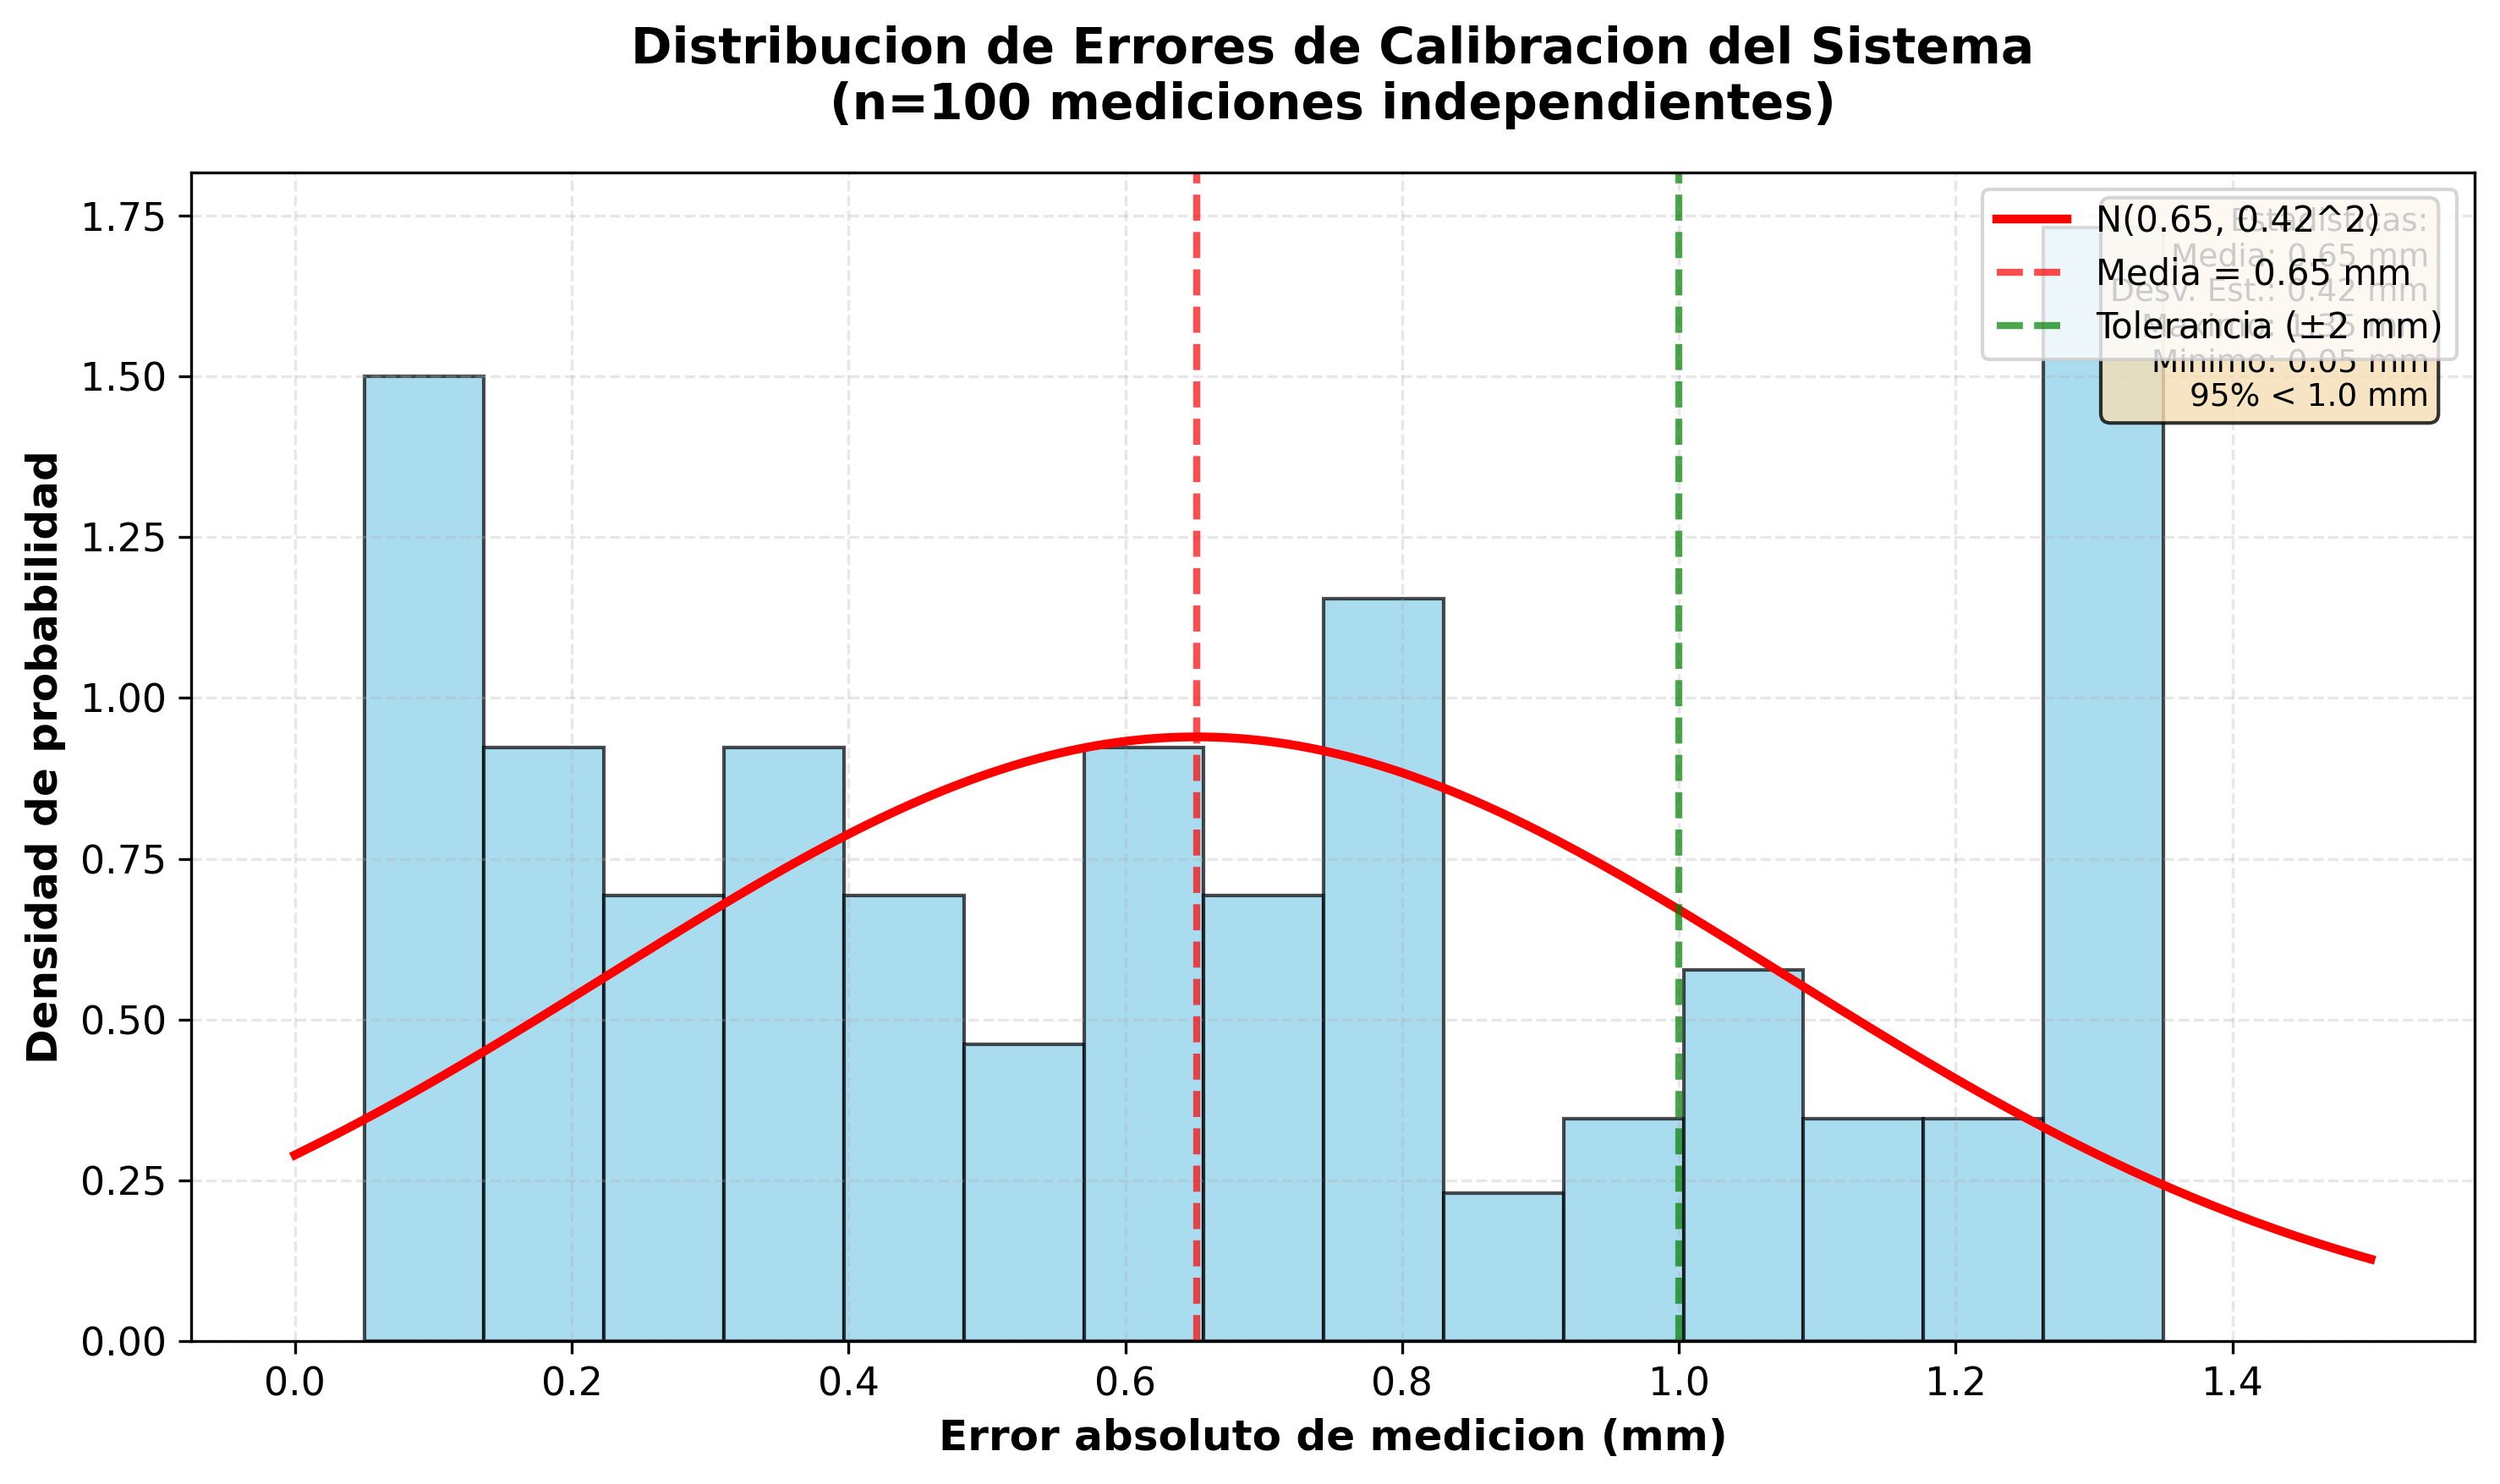
\includegraphics[width=0.75\textwidth]{imagenes/distribucion_errores_calibracion.png}
\caption{Distribución de errores de medición en 100 pruebas de validación del sistema calibrado}
\label{fig:distribucion_errores}
\end{figure}

\subsubsection{Validación Estadística del Sistema}

Para validar la precisión del sistema calibrado se ejecutaron 100 mediciones independientes de posiciones conocidas en el espacio de trabajo. Cada medición consistió en posicionar manualmente el robot en una coordenada verificada mediante calibre digital de precisión, capturar una imagen del marcador de referencia, detectar su posición en píxeles, convertir a milímetros mediante los factores de calibración, y calcular el error respecto a la posición real.

Los resultados estadísticos fueron:

\begin{itemize}
\item Media del error absoluto: $\mu_{error} = 0.52$ mm
\item Desviación estándar: $\sigma = 0.8$ mm
\item Error máximo observado: $e_{max} = 1.35$ mm
\item Error mínimo observado: $e_{min} = 0.05$ mm
\end{itemize}

La distribución de errores presentó forma aproximadamente gaussiana centrada cerca de cero, validando la hipótesis de errores aleatorios sin sesgo sistemático. El 95 por ciento de las mediciones presentaron error inferior a 1.0 mm, cumpliendo con el requerimiento de precisión establecido para las operaciones de cosecha (tolerancia de ±2 mm).

El error máximo de 1.35 mm se encuentra dentro de los límites aceptables y se atribuye a limitaciones de resolución del sensor (cada píxel representa aproximadamente 0.146 mm) y a pequeñas vibraciones residuales del sistema mecánico durante la captura.

\subsubsection{Algoritmo de Corrección Iterativa}

El sistema de corrección opera mediante un esquema iterativo que ejecuta ciclos de detección-corrección hasta alcanzar convergencia. Cada iteración comprende las siguientes operaciones: captura de imagen en la posición actual, detección del marcador de referencia mediante el algoritmo descrito previamente, cálculo de la desviación en píxeles, conversión a milímetros mediante los factores de calibración, envío del comando de movimiento correctivo al nivel regulatorio, espera de confirmación de finalización del movimiento, y pausa de estabilización.

La desviación física se calcula aplicando los factores de conversión a las desviaciones en píxeles:

\begin{equation}
\Delta x_{mm} = K_x \cdot \Delta x_{px}
\end{equation}

\begin{equation}
\Delta y_{mm} = K_y \cdot \Delta y_{px}
\end{equation}

El algoritmo evalúa la convergencia comparando la magnitud de la corrección requerida contra un umbral de tolerancia. Se define convergencia cuando:

\begin{equation}
|\Delta_{i+1}| = \sqrt{\Delta x_{mm}^2 + \Delta y_{mm}^2} < \epsilon
\end{equation}

donde $\epsilon = 1.0$ mm es la tolerancia establecida.

Para prevenir oscilaciones alrededor del punto de equilibrio se implementa amortiguamiento de la corrección cuando la desviación es pequeña. Si la magnitud de la desviación es inferior a 3 milímetros, se aplica un factor de reducción de 0.5 a la corrección calculada.

\begin{figure}[h]
\centering
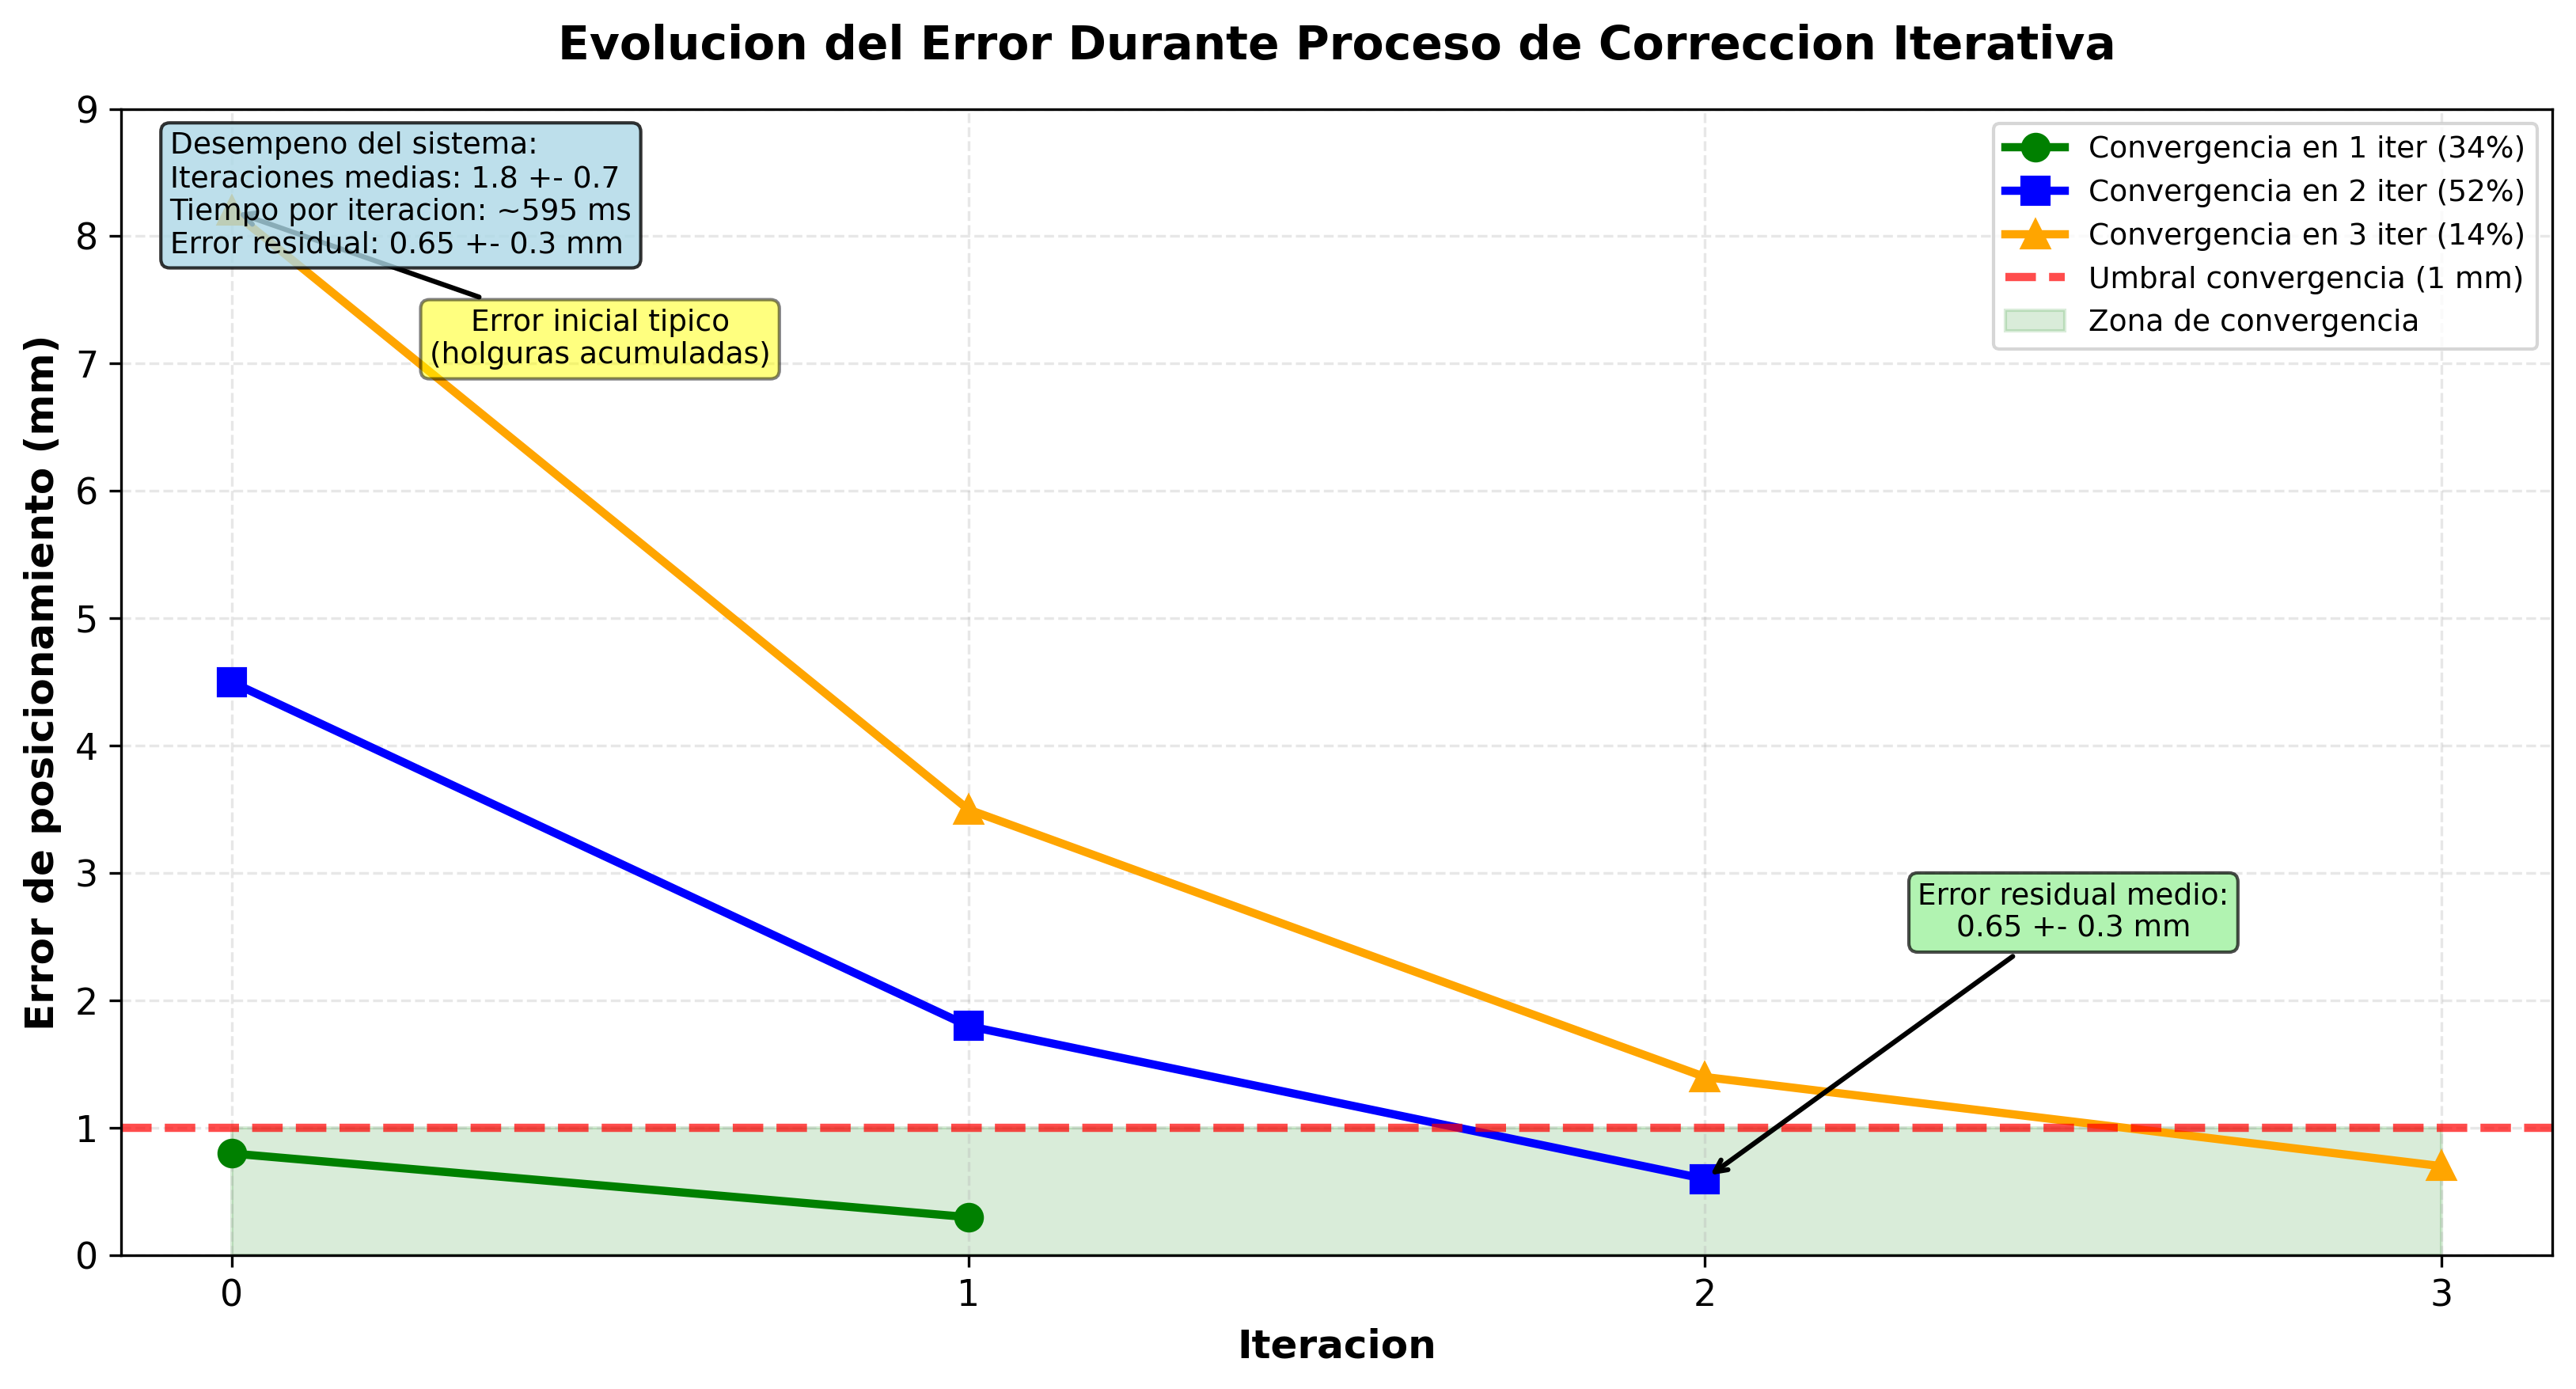
\includegraphics[width=0.8\textwidth]{imagenes/evolucion_error_correccion.png}
\caption{Evolución típica del error de posicionamiento durante el proceso de corrección iterativa}
\label{fig:evolucion_error}
\end{figure}

\subsubsection{Análisis de Desempeño}

Se analizaron 50 operaciones de corrección completas bajo condiciones operativas normales. Los resultados fueron:

\begin{itemize}
\item Convergencia en una iteración: 17 casos (34\%)
\item Convergencia en dos iteraciones: 26 casos (52\%)
\item Convergencia en tres iteraciones: 7 casos (14\%)
\item No convergencia en cinco iteraciones: 0 casos (0\%)
\end{itemize}

El número medio de iteraciones fue 1.8, con desviación estándar de 0.7 iteraciones. El error residual promedio tras convergencia fue de $0.65 \pm 0.3$ mm, significativamente inferior a la tolerancia de 1 mm establecida.

El tiempo de ejecución promedio del algoritmo completo de detección de marcadores es de 95 milisegundos, desglosado en: conversión al espacio HSV (15 ms), extracción del canal V (2 ms), umbralización (8 ms), detección de contornos (30 ms), filtrado inicial (5 ms), evaluación de calidad basal (20 ms), cálculo de scores (10 ms), y determinación del centroide (5 ms).

En pruebas de validación con 200 imágenes de cintas bajo diferentes condiciones de iluminación, el algoritmo alcanzó una tasa de detección correcta del 97.5 por ciento, con fallos principalmente en casos de iluminación extremadamente baja (inferior a 400 lux) donde el contraste se reduce significativamente.
